\section{Query Modulated Models Capacity \label{sec:additional-figures-query-mod-simultaneous}}

\begin{figure}[!htb]
% \vspace{-0.225in}
\centering
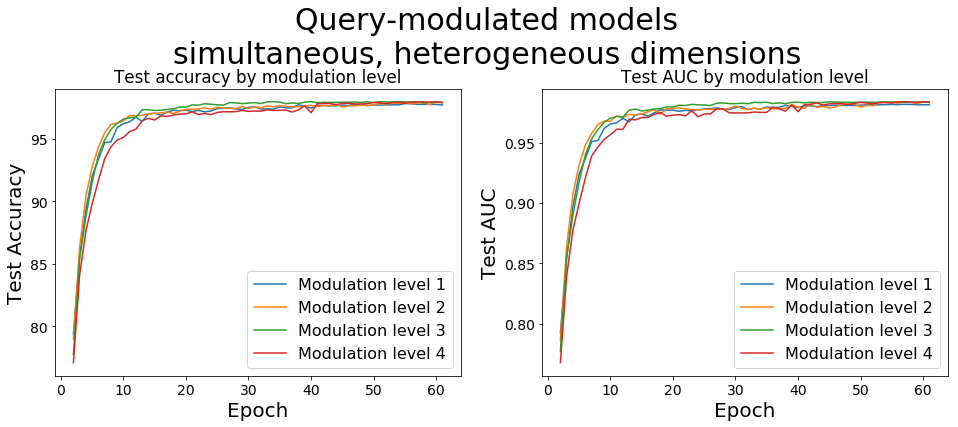
\includegraphics[width=\linewidth]{ch-results/figures/query_mod_simultaneous/query_mod_only.png}
\caption[Query-modulated models on simultaneous, heterogeneous dimensions.]{ {\bf Query-modulated models on simultaneous, heterogeneous dimensions.} This plot matches \ref{fig:results-query-mod-simultaneous-baseline-comparison}, but removes the baseline model, comparing only the four query-modulated ones. These models are still fairly inseparable.}
\label{fig:results-query-mod-simultaneous-query-mod-only}
% \vspace{-0.2in}
\end{figure}

\begin{figure}[!htb]
% \vspace{-0.225in}
\centering
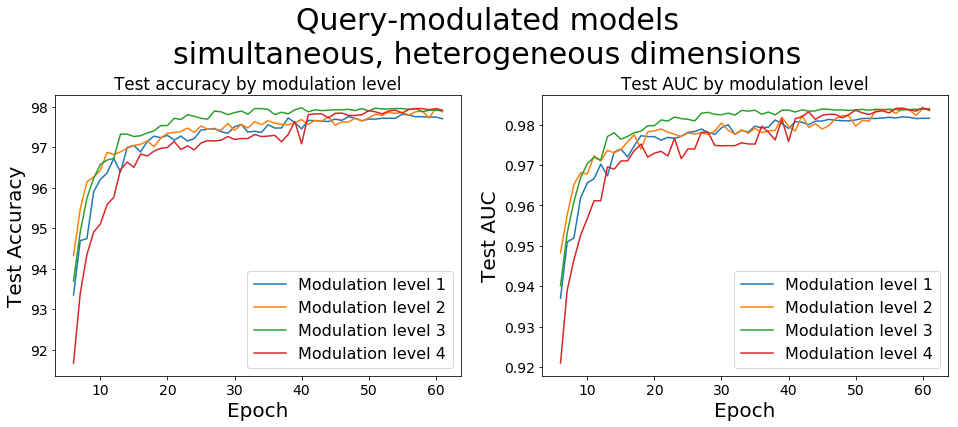
\includegraphics[width=\linewidth]{ch-results/figures/query_mod_simultaneous/query_mod_zoomed.png}
\caption[Zoomed-in version of \ref{fig:results-query-mod-simultaneous-query-mod-only}.]{ {\bf Zoomed-in version of \ref{fig:results-query-mod-simultaneous-query-mod-only}.} To attempt to better distinguish between query-modulated models, we examine them starting from their performance after the fifth training epoch. They still appear very close to even, with a slight advantage starting around epoch 15 to the model modulating at the third convolutional layer group.}
\label{fig:results-query-mod-simultaneous-query-mod-zoomed}
% \vspace{-0.2in}
\end{figure}
